\chapter{Results}
\label{ch:result}


In this chapter we will discuss the results retrieved after applying our LDA implementation. Section \ref{results:evaluation measures} defines the 4 different evaluation measures. In section \ref{results:modelresults} our results will be shown. Furthermore section \ref{results:parameter tuning} present the tuning results.

\section{Model results}\label{results:modelresults}


\begin{figure}[h]
    \centering
    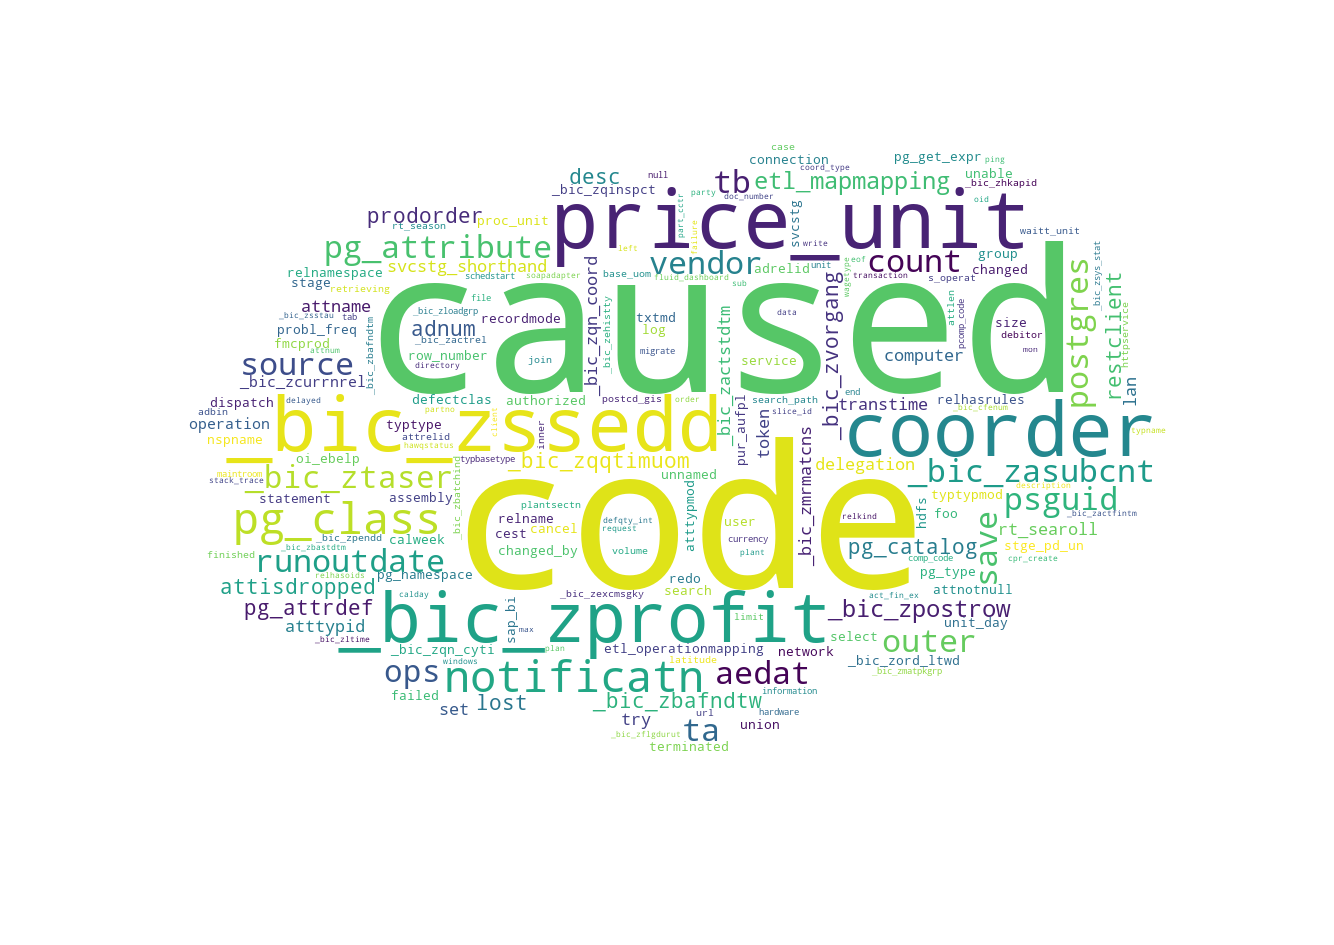
\includegraphics[width=15cm, height=8cm]{figures/wc.png}
    \caption{A wordcloud containing terms found in clusters}
    \label{fig:worldcloud}
\end{figure}

\begin{comment}

The model used is ofcourse LDA.

\end{comment}

\begin{comment}
# Time complexity is (n_samples * iterations)

n_components = 3 #10
alpha = float(5)/float(n_components)
eta = 0.01

batch_size = 4096 

kappa = 0.5
tau = 64
    
# n_docs_per_job = 10000
n_jobs = -1

#Samples
total_samples = 426905
n_samples = 4000 #2000
n_features = 1694 #100

max_iterations = 100
test_mode = 'online'
max_e_steps = 5
eval_every = 10


\end{comment}

\begin{table}[h]
\centering
 \begin{tabular}{|l|l| l|} 
 \hline
 Parameter & value & description \\ 
 \hline
 $\alpha$ (alpha) & 5/Number of topics & \\  
 $\beta$ (beta) & 0.1 &\\
 batch size  & 4096 &\\
 $\kappa$ (kappa) & 0.5 &\\
 $\tau$ (tau) & 64 &\\
 n docs per job & 10000&\\
 n jobs & -1 &\\
 Total samples & 426905&\\
 n samples & 4000 &\\
 n features & 1694 & \\
 max iteration & 100 &\\
 test mode & Online &\\
 max e steps & 5 &\\
 eval every & 10 &\\
 \hline
 \end{tabular}
\caption{Parameter settings}
\label{tab:table2}
\end{table}


\section{Graphs of results}



\begin{comment}
Visualizing the messages is really fun!
\end{comment}

\section{Contribution}\label{results:contribution}



\begin{comment}
I dont think I contributed a lot to the research in this area, but I learned a lot right??
\end{comment}
